\chapter{التخليق الكلي: الاستراتيجية والطرق الكلاسيكية}\label{ch:b3:total-synthesis}

عُزل الدواء المضاد للسرطان باكليتاكسيل أول مرة من لحاء الطقسوس
الباسيفيكي، وهو شجرة بطيئة النمو؛ وكان نزع اللحاء يقتل الشجرة، فكانت الكميات المتاحة
أبعد ما تكون عما يحتاج إليه المرضى. فأجاب الكيميائيون بطريقتين: تخاليق
كلية، بيّنت أن الجزيء يمكن بناؤه من مواد انطلاق بسيطة
لكنها كانت أطول بكثير من أن تصلح للإنتاج، \omterm{def:b3:total-synthesis:total}{وتخليق جزئي} انطلاقًا من مركب
قريب يُستخلص من أوراق طقسوس شائع، وهي متجددة.
ويتناول هذا الفصل كيف تُقيَّم مثل هذه الطرق وتُصمَّم: كيف تتضاعف المردودات،
ولماذا يربح التقارب، وما كلفة المجموعات الحامية، وأي الروابط
تُكوَّن أولًا، وثلاثة تخاليق بارزة تُقرأ بهذه الأدوات.

\begin{recall}
عالج مجلد السنة الثانية التحليل التخليقي الراجع (الجزيء الهدف، 
والفك، والسنثون، والمكافئ التخليقي، وتحويل المجموعة
الوظيفية)، والمجموعات الحامية المتعامدة، والتفاعل الألدولي، 
وحلقنة روبنسون، وتفاعل فيتيغ وكيمياء الإيمينيوم؛ وعالج مجلد السنة الأولى
المجموعات الحامية والمردودات. وقدّمت \cref{ch:b3:asymmetric-synthesis}
و\cref{ch:b3:pericyclic} و\cref{ch:b3:homogeneous-catalysis}
الخطوات الأساسية الحديثة.
\end{recall}

\begin{omfigure}
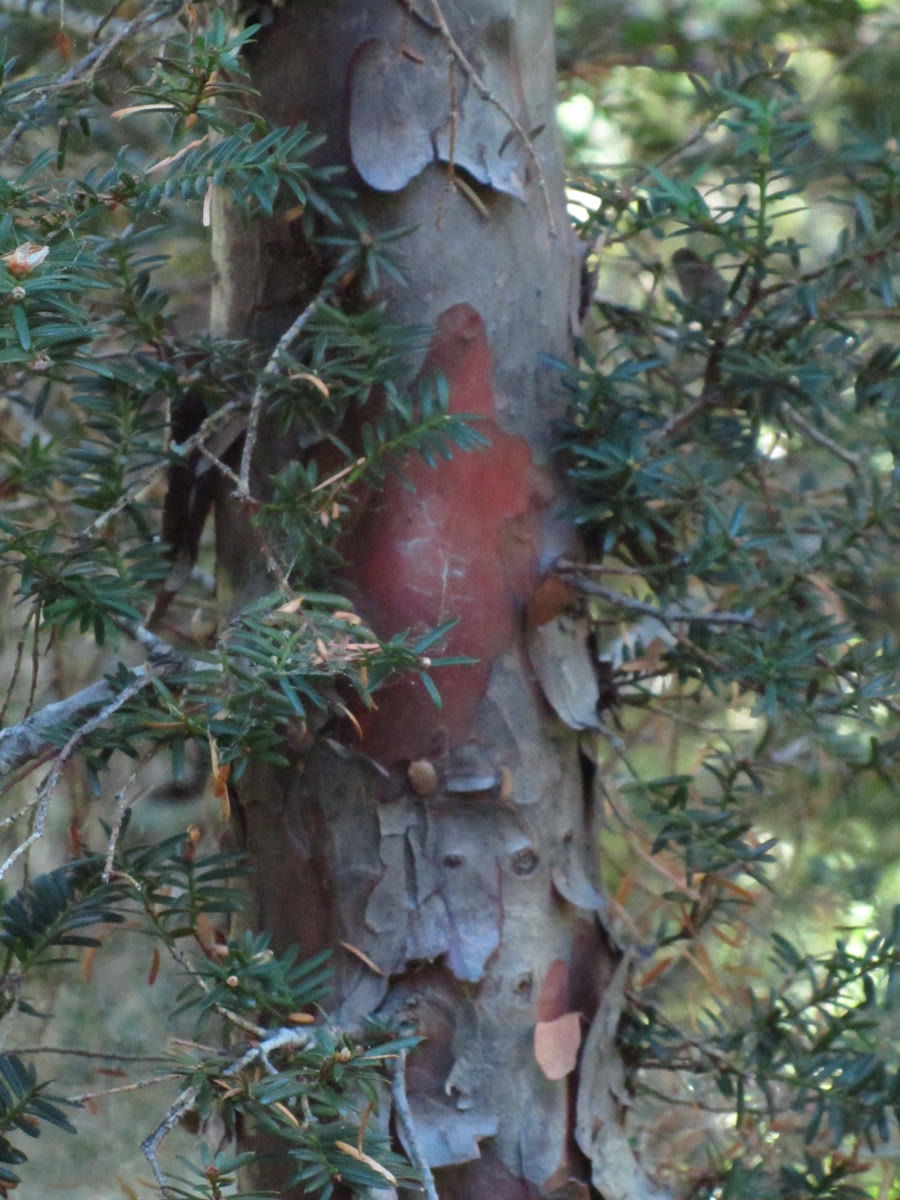
\includegraphics[width=0.32\linewidth]{images/book4/pacific-yew.jpg}

{\small لحاء الطقسوس الباسيفيكي وأوراقه، المصدر الأول للباكليتاكسيل.
الصورة: JOE BLOWE، CC BY-SA 2.0.}
\end{omfigure}

\section{قياس تخليق}

\begin{definition}[التخليق الكلي]\label{def:b3:total-synthesis:total}
\emph{التخليق الكلي}\index{تخليق كلي} يصنع جزيئًا معقدًا، يكون غالبًا
ناتجًا طبيعيًا، من مركبات تجارية بسيطة. و\emph{التخليق
الشكلي}\index{تخليق شكلي} يصنع وسيطًا في تخليق كلي سابق،
فيكمل الطريق على الورق. و\emph{التخليق الجزئي}\index{تخليق جزئي}
ينطلق من مركب طبيعي قريب سلفًا من الهدف.
\end{definition}

\begin{definition}[بنية الطريق]\label{def:b3:total-synthesis:architecture}
في \emph{التخليق الخطي}\index{تخليق خطي} تعمل كل خطوة على
ناتج الخطوة السابقة؛ وفي \emph{التخليق المتقارب}\index{تخليق متقارب}
تُصنع شظايا منفصلة على التوازي وتُوصل متأخرًا. 
و\emph{أطول تسلسل خطي}\index{أطول تسلسل خطي} (LLS) هو
أكبر عدد من الخطوات من أي مادة انطلاق إلى الهدف. 
و\emph{المردود الإجمالي}\index{مردود إجمالي} هو كمية الهدف المحصل عليها
مقسومةً على كمية مادة الانطلاق المحدِّدة.
\end{definition}

\begin{proposition}[المردود الإجمالي]\label{prop:b3:total-synthesis:overall-yield}
من أجل تسلسل من الخطوات مردوداتها $y_1, \dots, y_n$، يكون \omterm{def:b3:total-synthesis:architecture}{المردود الإجمالي} $Y = \prod_i y_i$.
\end{proposition}

\begin{proof}
تحوّل كل خطوة الكمية التي تتلقاها إلى $y_i$ مرة منها من الناتج؛ 
والكمية التي تبلغ الهدف هي كمية الانطلاق مضروبة في كل عامل على
التوالي.
\end{proof}

\begin{proposition}[التقارب]\label{prop:b3:total-synthesis:convergent}
للطريق المكوّن من $n = 2m + 1$ خطوة ذات مردود متساوٍ $y$، المبني على فرعين من $m$ خطوة تصلهما
خطوة اقتران واحدة، \omterm{def:b3:total-synthesis:architecture}{المردود الإجمالي} $y^{m+1}$ على امتداد \omterm{def:b3:total-synthesis:architecture}{أطول تسلسل خطي} فيه،
مقابل $y^{2m+1}$ للطريق الخطي ذي الخطوات نفسها.
\end{proposition}

\begin{proof}
يُصنع كل فرع على حدة، من الكمية اللازمة من مادة الانطلاق: فتمر
مادة كل فرع عبر $m$ خطوة ثم عبر الاقتران، أي $m + 1$
عاملًا $y$. وفي الطريق الخطي تمر المادة عبر الخطوات $2m + 1$ كلها. ومن أجل $m = 10$
و$y = 0.90$: 31\,\% مقابل 11\,\%.
\end{proof}

\begin{omfigure}
\begin{tikzpicture}
\begin{axis}[width=0.7\linewidth, height=5.8cm, xmin=0, xmax=30, ymin=0, ymax=1.02,
  axis lines=left, xlabel={\foreignlanguage{arabic}{عدد الخطوات $n$}}, ylabel={\foreignlanguage{arabic}{المردود الإجمالي}},
  tick label style={font=\scriptsize}, label style={font=\small},
  legend style={font=\scriptsize, draw=none, at={(1.03,0.5)}, anchor=west}, legend cell align=left]
\addplot[color=omDef, thick] table[x=n, y=y95] {figdata/out/bachelor-3-overall-yield.dat};
\addlegendentry{\foreignlanguage{arabic}{95\,\% لكل خطوة}}
\addplot[color=omMeth, thick] table[x=n, y=y90] {figdata/out/bachelor-3-overall-yield.dat};
\addlegendentry{90\,\%}
\addplot[color=omThm, thick] table[x=n, y=y80] {figdata/out/bachelor-3-overall-yield.dat};
\addlegendentry{80\,\%}
\addplot[color=omMeth, thick, dashed, mark=*, mark size=1pt] table[x=n, y=y90] {figdata/out/bachelor-3-overall-yield-b.dat};
\addlegendentry{\foreignlanguage{arabic}{90\,\%، متقارب}}
\end{axis}
\end{tikzpicture}

{\small \omterm{def:b3:total-synthesis:architecture}{المردود الإجمالي} بدلالة عدد الخطوات من أجل ثلاثة مردودات للخطوة
(بالخط المتصل: طرق خطية)، ومن أجل طرق متقاربة بمردود 90\,\% للخطوة (فرعان
متساويان يوصلان في خطوة أخيرة؛ بالمتقطع). وعشرون خطوة بمردود 90\,\% تُبقي 12\,\%؛ 
والخطوات نفسها مرتبةً على نحو متقارب تُبقي نحو ثلاثة أضعاف ذلك.}
\end{omfigure}

\begin{omfigure}
\begin{tikzpicture}[font=\scriptsize, >=Stealth, node distance=0.9cm,
  st/.style={circle, draw, fill=omDef!15, minimum size=4mm, inner sep=0pt}]
  \foreach \i in {0,...,6} { \node[st] (l\i) at (\i*0.9,1.6) {}; }
  \foreach \i in {0,...,5} { \pgfmathtruncatemacro\j{\i+1} \draw[->] (l\i) -- (l\j); }
  \node[anchor=west] at (6.0,1.6) {\foreignlanguage{arabic}{خطي: 6 خطوات، \babelsublr{LLS 6}}};
  \foreach \i in {0,...,2} { \node[st] (a\i) at (\i*0.9,0.6) {}; \node[st] (b\i) at (\i*0.9,-0.6) {}; }
  \draw[->] (a0) -- (a1); \draw[->] (a1) -- (a2); \draw[->] (b0) -- (b1); \draw[->] (b1) -- (b2);
  \node[st, fill=omThm!25] (t) at (3.0,0) {};
  \draw[->] (a2) -- (t); \draw[->] (b2) -- (t);
  \node[anchor=west] at (3.4,0) {\foreignlanguage{arabic}{متقارب: 5 خطوات، \babelsublr{LLS 3}}};
\end{tikzpicture}

{\small أشجار الطرق: كل دائرة مركب، وكل سهم خطوة. يمرر الطريق الخطي
كل مادته عبر كل خطوة؛ أما الطريق المتقارب فيصنع شظيتين
جنبًا إلى جنب ثم يقرنهما، فيكون \omterm{def:b3:total-synthesis:architecture}{أطول تسلسل خطي} فيه أقصر.}
\end{omfigure}

\begin{definition}[الاقتصادات والمثالية]\label{def:b3:total-synthesis:economy}
\emph{الاقتصاد في الخطوات}\index{اقتصاد في الخطوات} هو السعي إلى بلوغ الهدف بأقل
عدد ممكن من الخطوات؛ و\emph{الاقتصاد في المجموعات الحامية}\index{اقتصاد في المجموعات الحامية}،
هو السعي إلى استعمال أقل عدد ممكن من خطوات الحماية ونزعها. 
و\emph{مثالية}\index{مثالية} الطريق هي نسبة خطواته التي
تبني الهيكل أو تُحدث تغييرًا لازمًا في مستوى الأكسدة:
$(\text{خطوات البناء} + \text{خطوات الأكسدة والاختزال الاستراتيجية})/(\text{مجموع الخطوات})$.
\end{definition}

\begin{proposition}[مثالية الطريق]\label{prop:b3:total-synthesis:ideality}
الطريق في وعاء واحد الذي لا يكوّن إلا روابط الهيكل مثاليته 100\,\%؛ وكل خطوة حماية،
أو نزع حماية، أو تحويل للمجموعة الوظيفية، أو أكسدة واختزال غير استراتيجية
تخفضها.
\end{proposition}

\begin{proof}
مباشرة من التعريف: فهذه الخطوات تضاف إلى المقام دون أن تضاف
إلى البسط.
\end{proof}

\section{المجموعات الحامية واقتصادها}

تكلّف كل مجموعة حامية خطوتين على الأقل، والكواشف اللازمة لوضعها 
ونزعها، والمادة المفقودة في كلتيهما. فطريق من ثماني خطوات بمردود 90\,\% يحتفظ
بنسبة 43\,\% من مادته؛ وإضافة حمايتين ونزعي حماية بمردود 95\,\% لكل منها
تهبط به إلى 35\,\%. وتُختار المجموعات الحامية متعامدة، بحيث يمكن نزع كل منها
دون المساس بالأخرى؛ والأفضل من ذلك أن يُرتَّب تسلسل الخطوات
بحيث لا تكون المجموعة التفاعلية موجودة، أو لم تُكشف بعد، حين
كانت ستتداخل: فالتخاليق الخالية من المجموعات الحامية هدف، لا طرفة.

\begin{method}[قراءة تخليق كلي]\label{met:b3:total-synthesis:analyse}
\begin{enumerate}
  \item عيّن حلقات الهدف ومراكزه الفراغية ومجموعاته الحساسة.
  \item أوجد الفكوك الأساسية والتفاعلات التي تكوّنها في الاتجاه
        الأمامي (\omterm{def:b3:total-synthesis:strategic-bond}{الروابط الاستراتيجية}).
  \item عُدّ الخطوات وأوجد \omterm{def:b3:total-synthesis:architecture}{أطول تسلسل خطي}؛ ولاحظ درجة التقارب.
  \item لاحظ كيف يُثبَّت كل مركز فراغي (تحكم الركيزة، مساعد، حفاز،
        \omterm{def:b3:asymmetric-synthesis:chiral-pool}{مخزون كيرالي}).
  \item عدّد المجموعات الحامية والخطوات غير \omterm{def:b3:total-synthesis:economy}{المثالية} الأخرى؛ واحسب \omterm{def:b3:total-synthesis:architecture}{المردود
        الإجمالي} \omterm{def:b3:total-synthesis:economy}{والمثالية}.
\end{enumerate}
\end{method}

\begin{method}[عدّ الخطوات]\label{met:b3:total-synthesis:count}
\begin{enumerate}
  \item الخطوة عملية واحدة تنتهي بناتج معزول (أو معالَج على الأقل)؛
        والتسلسل في وعاء واحد دون عزل يُعدّ خطوة واحدة.
  \item عُدّ كل الخطوات للمجموع؛ ومن أجل \omterm{def:b3:total-synthesis:architecture}{أطول تسلسل خطي}، اتبع أطول مسار من
        مركب تجاري إلى الهدف.
  \item اضرب المردودات على امتداد \omterm{def:b3:total-synthesis:architecture}{أطول تسلسل خطي} للحصول على \omterm{def:b3:total-synthesis:architecture}{المردود الإجمالي}.
\end{enumerate}
\end{method}

\section{الروابط الاستراتيجية والخطوات الأساسية لتكوين الحلقات}

\begin{definition}[الرابطة الاستراتيجية]\label{def:b3:total-synthesis:strategic-bond}
\emph{الرابطة الاستراتيجية} في هدف\index{رابطة استراتيجية} رابطة يبسّط
فكها الهدف أكثر ما يكون، عادةً بشطر نظام حلقي
أو بإزالة عدة مراكز فراغية دفعة واحدة، ويستطيع تفاعل موثوق
تكوينها.
\end{definition}

تفاعلات تكوين الحلقات التي تكوّن رابطتين أو عدة مراكز فراغية دفعة واحدة
هي عُدّة العمل الأساسية: تفاعل ديلز--ألدر (رابطتا C--C، وحتى أربعة
مراكز فراغية، على نحو نوعي فراغيًا، \cref{ch:b3:pericyclic})، وحلقنة
روبنسون (حلقة سداسية على كيتون)، \omterm{def:b3:homogeneous-catalysis:metathesis}{والإبدال المغلق للحلقة}
(\cref{ch:b3:homogeneous-catalysis}) للحلقات المتوسطة والكبيرة، والتفاعلات الشلالية.

\begin{definition}[التفاعل الشلالي]\label{def:b3:total-synthesis:cascade}
\emph{التفاعل الشلالي}\index{تفاعل شلالي} تسلسل من
التحولات تُنشئ فيه كل خطوة الوظيفة اللازمة للخطوة التالية،
دون عزل الوسائط أو إضافة كواشف.
\end{definition}

\begin{definition}[التخليق المحاكي للطبيعة الحيوية]\label{def:b3:total-synthesis:biomimetic}
\emph{التخليق المحاكي للطبيعة الحيوية}\index{تخليق محاك للطبيعة الحيوية} يحاكي الطريق
الذي يُعتقد أن الكائن الحي يصنع به ناتجًا طبيعيًا.
\end{definition}

ألهم تحلّقُ أكسيد السكوالين إلى اللانوستيرول في الخلايا، بأربع حلقات وسبعة
مراكز فراغية في شلال إنزيمي واحد، تحلّقاتِ البولي إين لدى
ويليام جونسون، التي يغلق فيها كاتيون يبدأ عند أحد طرفي بولي إين مصمم بعناية
حلقةً بعد حلقة عبر حالات انتقالية شبيهة بالكرسي، فيثبّت
الالتحامات الحلقية \textit{trans} في الستيرويدات.

\section{طرق بارزة}

\begin{definition}[تفاعل مانيخ]\label{def:b3:total-synthesis:mannich}
\emph{تفاعل مانيخ}\index{تفاعل مانيخ} هو إضافة إينول
أو إينولات إلى أيون إيمينيوم، يُصنع في الموضع من ألدهيد وأمين أولي أو
ثانوي، فيعطي مركبًا كربونيليًا $\beta$-أمينيًا.
\end{definition}

في سنة 1917 صنع روبرت روبنسون التروبينون، النواة الثنائية الحلقة للأتروبين 
والكوكايين، في وعاء واحد من ثلاثة مكوّنات بسيطة في الماء، متخيلًا أن
النبات قد يبنيه بالطريقة نفسها:
$\ce{C4H6O2 + CH3NH2 + C5H6O5 -> C8H13NO + 2CO2 + 2H2O}$ (يعطي السكسينالدهيد والميثيل أمين 
وحمض الأسيتون ثنائي الكربوكسيليك التروبينون).

\begin{omfigure}
\begin{tikzpicture}[font=\small, >=Stealth]
  \node[align=center] at (-0.5,0) {$\ce{OHC-CH2CH2-CHO}$\\ $+\ \ce{CH3NH2}$\\ $+\ \ce{HO2C-CH2-CO-CH2-CO2H}$};
  \draw[->, thick] (3.0,0) -- (4.7,0) node[midway, above, font=\scriptsize] {\foreignlanguage{arabic}{ماء منظَّم}} node[midway, below, font=\scriptsize] {$-\ce{2CO2}$, $-\ce{2H2O}$};
  \begin{scope}[xshift=6.1cm, yshift=-0.2cm]
    \coordinate (c1) at (-1,0.3); \coordinate (c2) at (-0.8,-0.5); \coordinate (c3) at (0,-0.9);
    \coordinate (c4) at (0.8,-0.5); \coordinate (c5) at (1,0.3); \coordinate (c6) at (0.45,1.15);
    \coordinate (c7) at (-0.45,1.15); \coordinate (n) at (0,0.45);
    \draw[thick] (c1) -- (c2) -- (c3) -- (c4) -- (c5) -- (c6);
    \draw[thick] (c7) -- (c1);
    \draw[thick] (c6) -- (0.12,1.15); \draw[thick] (-0.12,1.15) -- (c7);
    \draw[thick] (c1) -- (n) -- (c5);
    \draw[thick] (n) -- (0,1.6) node[above, inner sep=1pt] {$\ce{CH3}$};
    \draw[thick, double, double distance=1.5pt] (c3) -- (0,-1.55) node[below, inner sep=1pt] {O};
    \node[fill=white, inner sep=0.5pt] at (n) {N};
    \node[font=\scriptsize, anchor=west] at (1.2,0.3) {\foreignlanguage{arabic}{التروبينون}};
  \end{scope}
\end{tikzpicture}

{\small تخليق روبنسون للتروبينون. يصل تفاعلا مانيخ، الأول
بين جزيئي والثاني مغلق للحلقة، المكوّنات الثلاثة؛ ثم
تغادر مجموعتا الحمض الكربوكسيلي اللتان جعلتا مجموعتي $\ce{CH2}$ المركزيتين قابلتين للتحول إلى إينول
في صورة ثنائي أكسيد الكربون. وفي الناتج الثنائي الحلقة يمتد جسر N-ميثيل عبر
الحلقة السباعية.}
\end{omfigure}

\begin{proposition}[التروبينون في وعاء واحد]\label{prop:b3:total-synthesis:tropinone}
تخليق التروبينون في وعاء واحد هو تفاعلا مانيخ يليهما
نزعان للكربوكسيل.
\end{proposition}

\begin{proof}[تعليل]
يعطي الميثيل أمين وإحدى مجموعتي الألدهيد في السكسينالدهيد أيون إيمينيوم؛ ويُضاف إليه
إينول حمض الأسيتون ثنائي الكربوكسيليك (\omterm{def:b3:total-synthesis:mannich}{تفاعل مانيخ} الأول). ويتكاثف الأمين الثانوي
المتكوّن مع مجموعة الألدهيد الثانية في أيون إيمينيوم
حلقي، يهاجمه الإينول الواقع على الجانب الآخر من الكيتون (\omterm{def:b3:total-synthesis:mannich}{تفاعل مانيخ} الثاني)،
فيغلق الحلقة الثنائية. ثم تفقد مجموعتا الحمض $\beta$-الكيتوني $\ce{CO2}$، كما تفعل الأحماض $\beta$-الكيتونية
عند التسخين المعتدل.
\end{proof}

جعل تخليق إلياس كوري للبروستاغلاندين $\mathrm F_{2\alpha}$ (1969) التحليل التخليقي الراجع
صريحًا. فثنائي حلقي[2.2.1]هبتينون مبني بتفاعل ديلز--ألدر يحمل
التشكيل النسبي لمستبدلات السيكلوبنتان؛ وتحوّله
\omterm{def:b3:radicals-carbenes:baeyer}{أكسدة باير--فيليغر} (\cref{ch:b3:radicals-carbenes}) 
ولكتنة يودية إلى لاكتون كوري، الذي تُربط منه السلسلتان الجانبيتان
بتفاعلات أولفنة. وقد خدم هذا اللاكتون منذ ذلك الحين أدوية بروستاغلاندينية كثيرة.

\begin{omfigure}
\begin{tikzpicture}[font=\small,
  box/.style={draw, rounded corners, align=center, fill=omDef!8, inner sep=4pt}]
  \node[box] (t) at (0,0) {\foreignlanguage{arabic}{البروستاغلاندين}\\ $\mathrm F_{2\alpha}$};
  \node[box] (l) at (4.4,0) {\foreignlanguage{arabic}{لاكتون كوري}\\ \foreignlanguage{arabic}{بأربعة}\\ \foreignlanguage{arabic}{مراكز فراغية}};
  \node[box] (b) at (9.2,0) {\foreignlanguage{arabic}{ثنائي حلقي \babelsublr{[2.2.1]}-}\\ \foreignlanguage{arabic}{هبتينون}};
  \node[box] (d) at (9.2,-2.4) {\foreignlanguage{arabic}{سيكلوبنتاديين}\\ \foreignlanguage{arabic}{مستبدل $+$ مكافئ}\\ \foreignlanguage{arabic}{للكيتين}};
  \draw[omretro] (t) -- (l) node[midway, above=3pt, font=\scriptsize] {\foreignlanguage{arabic}{أولفنات}};
  \draw[omretro] (l) -- (b) node[midway, above=3pt, font=\scriptsize, align=center] {\foreignlanguage{arabic}{لكتنة يودية،}\\ \foreignlanguage{arabic}{باير--فيليغر}};
  \draw[omretro] (b) -- (d) node[midway, right, font=\scriptsize] {\foreignlanguage{arabic}{ديلز--ألدر}};
\end{tikzpicture}

{\small التحليل التخليقي الراجع لكوري للبروستاغلاندين $\mathrm F_{2\alpha}$، بإيجاز (الأسهم المزدوجة: «يُصنع
من»). تُفك السلسلتان الجانبيتان أولًا؛ ويأتي السيكلوبنتان بمراكزه
الفراغية الأربعة من لاكتون، واللاكتون من كيتون ثنائي الحلقة،
والكيتون من تفاعل ديلز--ألدر يثبّت تشكيلها
النسبي.}
\end{omfigure}

يُصنع الأوسيلتاميفير، دواء الإنفلونزا، صناعيًا من حمض الشيكيميك، وهو
مركب من \omterm{def:b3:asymmetric-synthesis:chiral-pool}{المخزون الكيرالي} يُستخلص من اليانسون النجمي ثم صار يُنتج
بالتخمير: فحلقته السداسية ومراكزه الفراغية في مواضعها سلفًا.
ويحوّل الطريقُ ثنائيَّ الول الحلقي إلى إيبوكسيد، ويفتحه بالأزيد، ويغلق
أزيريدينًا ثم يفتحه بالأزيد من جديد، فيثبّت ذرتي النيتروجين في وضع
\textit{trans}؛ ثم تُتم الأستلة والاختزال العمل. ولأن أزيد الصوديوم 
والأزيدات العضوية سامة وقد تنفجر على النطاق الواسع، طُوّرت لاحقًا طرق
خالية من الأزيد.

\begin{omfigure}
\begin{tikzpicture}[font=\scriptsize, >=Stealth,
  box/.style={draw, rounded corners, align=center, fill=omMeth!8, inner sep=3pt}]
  \node[box] (a) at (0,0) {\foreignlanguage{arabic}{حمض \babelsublr{($-$)}-الشيكيميك}\\ \foreignlanguage{arabic}{من المخزون الكيرالي}};
  \node[box] (b) at (3.1,0) {\foreignlanguage{arabic}{إستر، كيتال،}\\ \foreignlanguage{arabic}{ميسيلات}};
  \node[box] (c) at (6.0,0) {\foreignlanguage{arabic}{إيبوكسيد}};
  \node[box] (d) at (8.6,0) {\foreignlanguage{arabic}{كحول أزيدي}};
  \node[box] (e) at (8.6,-1.5) {\foreignlanguage{arabic}{أزيريدين}};
  \node[box] (f) at (5.4,-1.5) {\foreignlanguage{arabic}{طليعة ثنائي الأمين \textit{trans}}\\ \foreignlanguage{arabic}{في صورة أزيد}};
  \node[box] (g) at (1.6,-1.5) {\foreignlanguage{arabic}{فوسفات}\\ \foreignlanguage{arabic}{الأوسيلتاميفير}};
  \draw[->] (a) -- (b); \draw[->] (b) -- (c); \draw[->] (c) -- (d) node[midway, above] {$\ce{N3-}$};
  \draw[->] (d) -- (e); \draw[->] (e) -- (f) node[midway, above] {$\ce{N3-}$};
  \draw[->] (f) -- (g) node[midway, below, align=center] {\foreignlanguage{arabic}{أستلة،}\\ \foreignlanguage{arabic}{اختزال}};
\end{tikzpicture}

{\small الأوسيلتاميفير من حمض الشيكيميك، المراحل الأساسية فقط: تُحفظ الحلقة الطبيعية 
ومراكزها الفراغية، وتُدخل ذرتا نيتروجين في وضع \textit{trans} إحداهما من الأخرى
بفتحين متتاليين لإيبوكسيد ولأزيريدين بالأزيد.}
\end{omfigure}

\section{من الاكتشاف إلى العملية الصناعية}

نادرًا ما يكون الطريق الذي يوفّر مليغرامات للاختبار الحيوي هو المستعمل
لصنع الأطنان. فكيميائيو العمليات يستكشفون الطرق من حيث الكلفة والسلامة والمتانة:
فيزيلون الكروماتوغرافيا لصالح البلورة، ويستبدلون الكواشف
الخطرة ودرجات الحرارة المنخفضة جدًا، ويقصّرون التسلسل، ويتحققون من السلامة
الحرارية لكل خطوة بالقياس الحراري، ويضعون مواصفات للشوائب.
وتلتقي هذه الخيارات بمقاييس \cref{ch:b3:green-industrial}.

\begin{inthelab}[من غرام واحد إلى كيلوغرام]
تُعاد خطوة أُجريت على غرام واحد في دورق مستدير القاع على عشرة غرامات في
مفاعل ذي غلاف مع محرّك علوي ومسبار حرارة في
السائل، مع إضافة الكاشف التفاعلي بسرعة مضبوطة ومراقبة
درجة الحرارة الداخلية: فالحرارة المنطلقة تكبر مع الحجم، أما المساحة التي
تزيلها فلا تكبر إلا كمربع الحجم الخطي. ولا تُجرى الخطوة على كيلوغرام إلا حين يكون تدفق الحرارة والمعالجة
(فصل الأطوار، والترشيح، والتجفيف) منضبطين.
\end{inthelab}

\begin{safety}{\ghs[0.62cm]{GHS06}\ghs[0.62cm]{GHS08}\ghs[0.62cm]{GHS09}}
% ledger: ghs4:NaN3
أزيد الصوديوم: قاتل إذا ابتُلع، شديد السمية للأحياء المائية؛ ومع الأحماض
يطلق حمض الهيدرازويك، وهو غاز سام ومتفجر، ومع الفلزات الثقيلة
(النحاس والرصاص في المصارف) يكوّن أزيدات متفجرة. وتُتلف النفايات
كيميائيًا، ولا تُصب في المصارف أبدًا.
\end{safety}

\begin{history}[روبنسون، وودوارد، كوري]
نال روبرت روبنسون جائزة نوبل في الكيمياء لسنة 1947 عن أعماله في
القلويدات وغيرها من النواتج النباتية؛ ولا يزال تخليقه للتروبينون سنة 1917
يُستشهد به لاقتصاده. وجعلت تخاليق روبرت وودوارد للكينين والكوليسترول 
والكلوروفيل، والفيتامين $\mathrm B_{12}$ مع ألبرت إشنموزر، التخليقَ الكلي فنًّا
(جائزة 1965). وصاغ إلياس كوري التحليل التخليقي الراجع صياغة منهجية ونال
جائزة 1990 عن نظرية التخليق العضوي ومنهجيته.
\end{history}

\section{تمارين}

\begin{exercise}[$\star$]\label{exo:b3:total-synthesis:1}
احسب \omterm{def:b3:total-synthesis:architecture}{المردود الإجمالي} لطريقين خطيين من 10 خطوات ومن 20 خطوة بمردود 90\,\% وبمردود 80\,\% لكل
خطوة.
\end{exercise}

\begin{exercise}[$\star$]\label{exo:b3:total-synthesis:2}
يصنع طريق الشظية A في خمس خطوات والشظية B في ثلاث، ويقرنهما، ثم
يحتاج إلى أربع خطوات أخرى حتى الهدف. أعطِ العدد الكلي للخطوات 
\omterm{def:b3:total-synthesis:architecture}{وأطول تسلسل خطي}.
\end{exercise}

\begin{exercise}[$\star$]\label{exo:b3:total-synthesis:3}
أعطِ ناتج \omterm{def:b3:total-synthesis:mannich}{تفاعل مانيخ} بين الأسيتون والفورمالدهيد 
وثنائي ميثيل أمين.
\end{exercise}

\begin{exercise}[$\star$]\label{exo:b3:total-synthesis:4}
أعطِ فكًّا من نوع ديلز--ألدر للمركب 4-أسيتيل سيكلوهكسين، والتفاعل
الأمامي.
\end{exercise}

\begin{exercise}[$\star\star$]\label{exo:b3:total-synthesis:5}
يجري طريق خطي من 21 خطوة بمردود 90\,\% لكل خطوة. احسب مردوده الإجمالي 
ومردود نسخة متقاربة بفرعين من 10 خطوات واقتران واحد.
\end{exercise}

\begin{exercise}[$\star\star$]\label{exo:b3:total-synthesis:6}
للطريق A اثنتا عشرة خطوة، منها 7 تكوّن روابط الهيكل و1 اختزال
استراتيجي؛ وللطريق B تسع خطوات، 7 منها هيكلية. احسب مثاليتيهما.
\end{exercise}

\begin{exercise}[$\star\star$]\label{exo:b3:total-synthesis:7}
يحتاج طريق من ثماني خطوات بمردود 90\,\% لكل خطوة إلى مجموعتين حاميتين، توضع كل منهما 
وتُنزع بمردود 95\,\%. احسب \omterm{def:b3:total-synthesis:architecture}{المردود الإجمالي} معهما ودونهما.
\end{exercise}

\begin{exercise}[$\star\star$]\label{exo:b3:total-synthesis:8}
لثلاثي ول مجموعة هيدروكسي أولية وأخرى ثانوية وثالثة ثالثية. اقترح
مجموعات حامية تتيح كشف كل منها بالتتابع، وظروف
نزعها.
\end{exercise}

\begin{exercise}[$\star\star$]\label{exo:b3:total-synthesis:9}
لماذا أُنتج الباكليتاكسيل \omterm{def:b3:total-synthesis:total}{بالتخليق الجزئي} لا بأي من تخاليقه
الكلية؟
\end{exercise}

\begin{exercise}[$\star\star\star$]\label{exo:b3:total-synthesis:10}
يتفاعل 2-ميثيل سيكلوهكسان-1،3-ديون مع ميثيل فينيل كيتون في حلقنة
روبنسون. عيّن خطوتي مايكل والألدول وأعطِ الإينون الثنائي الحلقة
المتكوّن (كيتون فيلاند--ميشر).
\end{exercise}

\begin{exercise}[$\star\star\star$]\label{exo:b3:total-synthesis:11}
بيّن أن الطريق المتقارب في \cref{prop:b3:total-synthesis:convergent} يحتفظ
بمادة أكثر بمقدار $y^{-m}$ مرة من الطريق الخطي، وقدّر هذا العامل من أجل $m = 5$ 
و$m = 15$ بمردود 90\,\%.
\end{exercise}

\begin{exercise}[$\star\star\star$]\label{exo:b3:total-synthesis:12}
في تحلّق بولي إين، لماذا تعطي الحالات الانتقالية الشبيهة بالكرسي التحامات حلقية \textit{trans}،
ولماذا يهم شكل كل رابطة مضاعفة (\textit{E} أو \textit{Z})؟
\end{exercise}

\section{مسألة: التروبينون في وعاء واحد}

\begin{problem}[{مسألة نهاية الأسبوع --- التروبينون في وعاء واحد: المكوّنات الثلاثة
والمعادلة الموزونة، وتفاعلا مانيخ، والمقارنة بطريق خطي
طويل، والكيمياء الفراغية للتروبينون ونواتج اختزاله}]
\label{pb:b3:total-synthesis:1}
% ledger: aw:C, aw:H, aw:N, aw:O
معطيات المسألة: يعطي التخليق في وعاء واحد، المُجرى في ماء منظَّم قرب pH 5،
التروبينون بمردود 42\,\%؛ ويحتاج طريق خطي أقدم إلى 14 خطوة بمردود متوسط 75\,\%.

\medskip\noindent\textbf{الجزء الأول --- المكوّنات والمعادلة.}
\begin{enumerate}
  \item أعطِ صيغ السكسينالدهيد والميثيل أمين وحمض الأسيتون ثنائي الكربوكسيليك
        والتروبينون.
  \item اكتب المعادلة الموزونة.
  \item احسب الكتل المولية للمتفاعلات وللتروبينون.
  \item احسب الاقتصاد الذري.
  \item لماذا يُستعمل حمض الأسيتون ثنائي الكربوكسيليك بدل الأسيتون؟
  \item لماذا يفيد التنظيم قرب pH متعادل؟
\end{enumerate}

\medskip\noindent\textbf{الجزء الثاني --- الآلية.}
\begin{enumerate}[resume]
  \item اكتب تكوّن أيون الإيمينيوم الأول.
  \item بيّن \omterm{def:b3:total-synthesis:mannich}{تفاعل مانيخ} الأول.
  \item كيف يتكوّن أيون الإيمينيوم الثاني؟
  \item بيّن \omterm{def:b3:total-synthesis:mannich}{تفاعل مانيخ} الثاني المغلق للحلقة.
  \item لماذا تغادر مجموعتا الحمض الكربوكسيلي في صورة $\ce{CO2}$؟
  \item عُدّ روابط C--C وC--N المتكوّنة.
\end{enumerate}

\medskip\noindent\textbf{الجزء الثالث --- وعاء واحد مقابل أربع عشرة خطوة.}
\begin{enumerate}[resume]
  \item احسب \omterm{def:b3:total-synthesis:architecture}{المردود الإجمالي} للطريق الخطي.
  \item احسب نسبة مردود الوعاء الواحد إليه.
  \item احسب \omterm{def:b3:total-synthesis:economy}{مثالية} الطريق في وعاء واحد.
  \item ما الذي يرجّح الطريق في وعاء واحد غير المردود؟
  \item لماذا يسمى التخليق في وعاء واحد محاكيًا للطبيعة الحيوية؟
  \item سمِّ صنفًا آخر من تفاعلات هذا الفصل يكوّن عدة روابط دفعة واحدة.
\end{enumerate}

\medskip\noindent\textbf{الجزء الرابع --- الكيمياء الفراغية.}
\begin{enumerate}[resume]
  \item هل التروبينون كيرالي؟ أوجد عنصر تناظره.
  \item لماذا تكون ذرتا الكربون عند رأسي الجسر مركزين فراغيين رغم ذلك؟
  \item يعطي اختزال الكيتون كحولين، التروبين والسودوتروبين. ما
        العلاقة بينهما؟
  \item هل التروبين والسودوتروبين كيراليان؟
  \item لماذا يقترب الهيدريد من مجموعة الكربونيل من أحد الوجهين تفضيليًا؟
  \item اذكر النتيجة: نسبة مردود الوعاء الواحد إلى \omterm{def:b3:total-synthesis:architecture}{المردود الإجمالي} للطريق
        الخطي.
\end{enumerate}
\end{problem}
